
\chapter{Méthode proposée}

L'objectif de notre méthode est d'avoir une reconnaissance multi-vues d'un ou plusieurs objets à la fois, capable d'intégrer le déplacement du robot pour résoudre des ambiguïtés et faux positifs. Pour incorporer les notions de vue et de transition entre elles, on s'utilise d'une représentation simple et suffisamment général basé sur les graphes d'aspect, couplé avec un dispositif de reconnaissance mono-vue classique capable d'estimer l'orientation de l'objet reconnu. Une suivi des objets et un traitement probabiliste intègre l'information motrice pour augmenter le taux de reconnaissance.

\section{Architecture générale}
L'approche cible une base mobile différentiel muni de capteurs proprioceptives odométiques et d'une caméra RGB-D. Les informations provenant des ces unités sont envoyés à une unité de traitement qui interprète les images reçus et compare cette interprétation avec une base de données contenue dans la mémoire. Dans le cas d'absence de correspondent, ce nouveau exemplaire peut être ajouté à la base de données et agrandir les connaissances d'objets existants dans l'environnement. 

L'architecture est illustrée dans \ref{fig:architecture} et permet à, la fois, de comprendre les dépendances entre les étapes de traitement, de même que, la nature du flux d'information entre modules.

\begin{figure}[H]
  \centering
  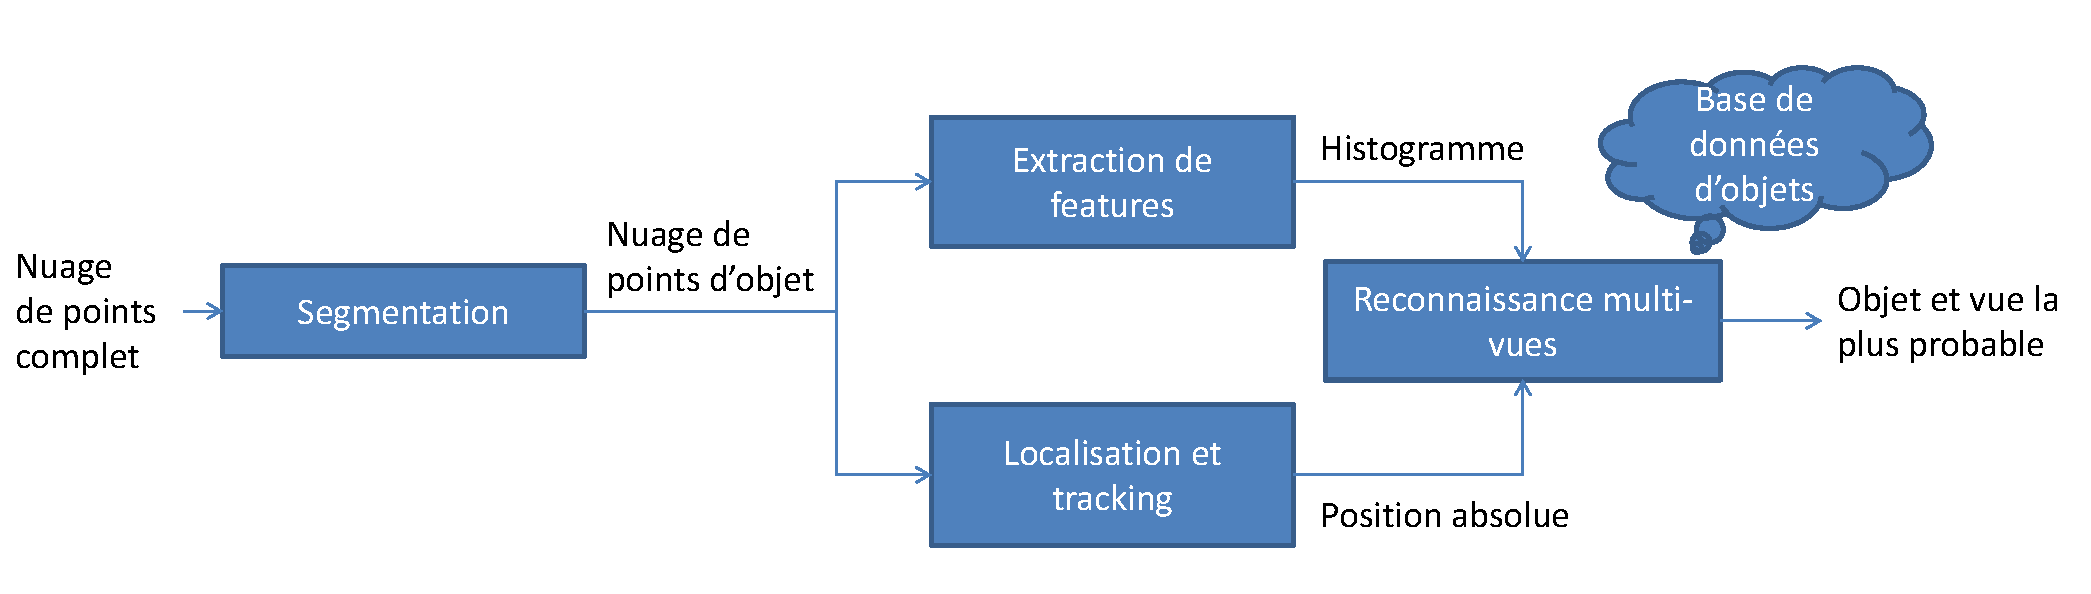
\includegraphics[width=\textwidth]{gen_arc.pdf}
  \caption{Architecture générale du système}
  \label{fig:architecture}
\end{figure}

Précisément, l'unité de traitement reçois une nuage brute provenant de la caméra et la mesure de rotation de roues du robot. La première partie du traitement vise nettoyer le nuage en segmentant des points des objets candidats de la scène, ce qui permet, déjà, d'enlever une partie non pertinent et envoyer à l'unité de extraction de features seulement des morceaux de l'image original qui respectent certains caractéristiques. Simultanément, un conversion de référentiel localise des objets dans le repère absolu de déplacement du robot. Puis, les positions des objets sont donnés au module de localisation et tracking qui suit les observations et les associes entre elles pour avoir une cohérence globale des positions. En dernière instance, les histogrammes de features , aussi comme, la position, dans la carte globale, de chaque objet sont utilisés pour pour reconnaitre les éléments de la scène et pour donner leur vue la plus probable à chaque instant de temps. 

Les prochaines sections dissèquent l'architecture de l'image \ref{fig:architecture}, en présentant le fond théorique derrière le fonctionnement de chaque sous module.

\section{Segmentation}

La segmentation consiste de la soustraction des objets d'une image brute, en autres mots, différencier les éléments non constituent du objet de lui-même. La compréhension de la continuité des objets est considérée comme un défi majeur dans le traitement d'image étant donné qu'une fois l'objet séparé du fond, la reconnaisse devient beaucoup plus évident. Une énorme partie de sa difficulté vient du fait de la projection de la scène dans le plan supprimer l'information
correspondant à distance. Les capteurs stéréoscopiques et infra-rouges ont recomposé cette absence d'information et simplifié énormément le traitement nécessaire pour obtenir des objets potentiels. Les cartes de profondeur pourraient être utilisées pour représenter cette nouvelle information, pourtant, encore plus naturelle, le concept de nuage de points propose une représentation spatial en trois dimensions de l'environnement capturé.

La démarche proposée par la littérature considère les objets comme des
ensembles de points définis par un seuil initial de proximité. Cette
définition est bien extensive et permet de représenter une énormité,
sinon tous, les objets. Néanmoins, définir ces ensembles dans une
image brute n'est pas tout à fait simple. En conséquence, un nouveau à
priori qui spécifie que les objets se placent sur des plans de
support, malgré plus restrictif que la définition d'avant, permet un
segmentation crédible.

\subsection{Algorithme}

La méthode de segmentation de l’algorithme Tabletop
se base exactement sur ces aprioris. Pour retrouver les objets posés
sur une table, l'algorithme recherche récursivement les plans de
support, où le plus important est pris comme la table. Autrement,
l'article \cite{caron2014neural} en partant du même principe, propose un
traitement pour le fond de la scène, où les plans orthogonaux à
normale du sol et de taille suffisamment grand sont considérés comme
des murs, orientés à segmentation d'objets dans les environnements
intérieurs. Ainsi, la dernière segmentation répond aux exigences du domaine de déplacement du robot: le
laboratoire de Thales, Theresis.\\

Plus spécifiquement, elle peut être découpée dans les étapes suivantes :
\begin{enumerate}
\item Soustraction du sol

\item Filtrage de points distants, considérés comme plus incertains.

\item Calcul de la normale des superficies comprises dans la scène

\item Élimination de murs, considérés comme de plans orthogonaux au
  sol de taille suffisamment grande, d'après un seuil.

\item Projection des points appartenant aux objets dans le plan du
  sol.

\item Détermination de l’enveloppe convexe correspondant au sol détecté.

\item Réduction de la densité de discrétisation pour accélérer l'étape
  de \textit{clustering}.

\item \textit{Clustering} des objets par l'algorithme \textit{point growing}

\item Calcul du centroïde et \textit{bouding boxes} 2D et 3D \\

\end{enumerate}

Une calibration initiale est nécessaire pour définir l'équation du
sol. Pour cela, on place le robot dans un endroit de façon que l'image
aperçue correspond majoritairement au sol. L’équation du plan plus
important, plus grand nombre de points dans le nuage, est extrait par
le RANSAC et sauvegardé dans un fichier texte. Une explication plus
détaillée sur les sous-méthodes utilisées pour chaque étape, telle
comme le RANSAC est présentée dans les annexes, ainsi comme une
discussion des paramètres utilisés.

\subsection{Restrictions} Les physiques de capteurs restreins les
types d'objet qui peuvent être aperçus et, ensuite, segmentés, soit à
cause de l'interaction avec les rayons infra-rouges, soit à cause de
résolution limitée des images mesurées. Dans l'autre côté, la
segmentation a ses propres contraints concernant le positionnement des
objets dans l'image et, principalement, la définition de sol et murs,
résultant dans les restrictions suivantes :\\

\begin{itemize}
\item L'objet se trouve par terre.
\item L'objet se trouve au centre de l'image.
\item Ambiant isolés de lumière infra-rouge.
\item L'objet n'est ni transparents et ni trop réflective.
\item Le sol où le robot se déplace n'est pas accidenté.
\item L'objet se trouve à une distance inférieure à 3 mètres.
\item L'objet est assez grand et dépasse le seuil d'appartenance au sol.\\

\end{itemize} 

Un grand nombre d'objets, entre chaises tables, écrans, boîtes en
carton, poubelles, de tailles et formes variés étaient testés et
peuvent être segmentés malgré les restrictions listées. Quelques
exemples de segmentation sont présentés dans les annexes pour illustrer
la capacité de segmentation.

\section{Descripteurs}

Le travail des descripteurs est, d'un côté, de comprendre les
caractéristiques intéressants et, d'un autre, de réduire la
dimensionnalité du espace traité, tandis que restant robuste à des
transformations affines et changement de luminosité. On classifie les
descripteurs selon la caractéristique qu'ils expriment. Une première
groupe sont les descripteurs géométriques qui essaient de traduire les
idées de courbure, forme et taille dans histogrammes, et sont intéressant
pour étudier les ambiguïtés de reconnaissance, un fois que la plus parts 
d'objet ont une certaine symétrie spatial.


En partant de l'hypothèse que la segmentation donné une bonne fragmentation des objets, on extrait des descripteurs globales à partir de les ensembles de points donnés par le première traitement. L'adoption du descripteur \textit{Viewpoint Feature Histogram} - VFH, entre tous proposés par la littérature, reflet l'intérêt d'avoir une distinction entre formes géométriques et entre points de vues. Une description détaillée du descripteur est rencontré dans les annexes.  

\section {Reconnaissance mono-vue} 

matching des descripteurs avec la base de données...

L'étape de classification correspond à la différentiation entre les
histogrammes caractéristiques de chaque vue de chaque objet. Cette
mesure pourrait être apprise, par exemple, avec un réseau de neurone
ou n'importe quel autre méthode classique de \textit{machine learning}.{\color{green}Le travail * three dimensional
  dof cluster vfh...* suggère l'utilisation de la mesure chi-squared
  similarité entre histogrammes accouplé au classificateur k plus
  proches voisins. }  Le grand avantage de ce classificateur c'est l'étape
d’apprentissage correspond à création d’un arbre de recherche,
construit d'après la comparaison croisée entre les éléments de la base,
que pour l'ordre de grandeur de la base de données envisagé, est
presque instantané. Distance plus naturel...

L'API de la librairie FLANN sur PCL permet l'utilisation directe du classificateur
K - plus proches voisins. L'implémentation permets l'utilisation de plusieurs
définitions de distance entre histogrammes. La définition par défaut, Chi-squared,
dont la formule est décrit dans la suite, semble être capable de bien différentier
les histogrammes d'entrés, $H_1$ et $H_2$, et était choisi comme la définition pour le classificateur.

$$d(H_1, H_2) = \sum _I \frac{\left(H_1(I)-H_2(I)\right)^2}{H_1(I)} $$

% Une étude des mesures de corrélation entre histogrammes peut être
% intéressant. Ces mesures sont classifié en deux classes : croisés et
% directs. La comparaison direct prend en compté différences par rapport
% à la même cellule de l’histogramme. Pendent que la comparaison croisée
% permet la comparaison entre cellules, par une matrice de
% corrélation. Les features géométriques ont des cellules bien définis
% et statiques, ainsi, semble plus naturel d'utiliser une comparaison
% \textit{bin-to-bin}.
% \subsection{bin-to-bin} Comparaison entres cellules équivalents
% \begin{itemize}
% \item Correlation :
% \item Intersection :
% \item Bhattacharyya distance :
% \end{itemize}

\section{Localisation et suivi d'objet}

\subsection{Définition de repères}

Se placer dans différents repères permettre d'avoir de référentiels plus naturels pour chaque type de composant du robot et pour les objets placés dans la scène. On défini quelques repères et conventions de base pour faciliter la localisation. D'abord le repère de la base du robot est orthonormale positive, où le déplacement ver l'avant correspond à l'axe $x$, vers la gauche à l'axe $y$ et ver le haut à l'axe $z$. Une deuxième référentielle de convention égale à celle d'avant positionne le capteur RGB-D par rapport au robot. Enfin, le dernière référentiel corresponde au repère optique du capteur orienté selon la convention usuelle pour les images avec l'axe $x$ orienté ver la droite et l'axe $y$ ver le bas et, enfin, l'axe $z$ vers l'avant. Ces trois repères permettent d'orienter tous les éléments aperçus par le robot dans l'environnement de façon pratique.

La \review{figure} illustre ces repères utilisés et les conventions décrits.

\subsection{Transformation de repères}

Ensuite, la transformation entre repères permet la passage de l'un à l'autre, pour avoir la position globale de l'objet d'après sa détection par la caméra. La transformation entre une base $a$ et une autre $b$ est faite par une matrice de rotation et translation classique, décrit en bas. 

\begin{equation*}
	\mathbf{R}^{a}_{b} = 
	\begin{bmatrix} 
	 	\cos \theta &  -\sin \theta & \Delta x \\ \sin \theta & \cos \theta & \Delta y \\ 0 & 0 & 1
	 \end{bmatrix}
\end{equation*}

où $\theta$ équivaut à la rotation entre les deux repères et $\Delta x$ et $\Delta y$ sont les translations linéaires entre eux.

\subsection{les bases mobiles}

\subsubsection{Estimation de l'odométrie}

Certains robots sont dotés de capteurs à estimer de façon
approximé sont déplacement. C'est aussi le cas du robot ciblé qui
possède encodeurs capables d'estimer la rotation angulaire des
roues. Une intégration, au sens mathématique, de la différence entre
l'odométrie entre deux intervalles de temps permet de retrouver la
position global du robot.

\begin{equation*}
	\begin{array}{rcl}
		x_t &=& x_{t-1} + \delta x_{t-1} * cos(\theta_{t-1}) - \delta y_{t-1} * sin(\theta_{t-1}) \\
		y_t &=& y_{t-1} + \delta x_{t-1} * sin(\theta_{t-1}) + \delta y_{t-1} * cos(\theta_{t-1}) \\
		\theta_t &=& \theta_{t-1} + \delta\theta_{t-1}
	\end{array}
\end{equation*}


Les plates-formes différentielles Une des configurations les plus utilisées pour les robots mobiles d’intérieur est la configuration différentielle qui comporte deux roues commandées indépendamment. Une ou plusieurs roues folles sont ajoutées à l’avant ou à l’arrière du robot pour assurer sa stabilité (Figure 4.1). Cette plate-forme est très simple à commander, puisqu’il suffit de spécifier les vitesses des deux roues, et permet de plus au robot de tourner sur place. Cette possibilité permet de traiter dans certains cas le robot comme un robot holonome, ce qui va simplifier la planification de déplacement et la commande du robot.

L’estimation du déplacement par odométrie est également très simple à partir de la mesure des vitesses de rotation des deux roues et . Les vitesses de translation v et de rotation sont en effet données par :

Ce type de plate-forme peut également être utilisé avec des chenilles ce qui fournit une capacité de franchissement de petits obstacles intéressante (Figure 4.1). Ces plates-formes peuvent ainsi être utilisées en extérieur ou dans des décombres. L’utilisation de chenilles conduit cependant à une odométrie très bruitée à cause du contact mal défini entre les chenilles et le sol qui glissent beaucoup, notamment lors des rotations. L’estimation de la direction par l’odométrie sur ce type de plates-formes est donc en général rapidement inutilisable.

\subsection{Filtre de Kalman }

La modélisation des objets entraîne le besoin initiale de les
localiser dans la scène pour, postérieurement, les identifier. À cause
de la divergence de l'odométrie, la mauvaise segmentation et le calcul
du centroïde de l'objet, la position estimée est fortement bruitée
ayant un écart type qui rend la suive et identification infaisable
lorsque plusieurs objets sont minimalement proches. Un filtre de
Kalman ayant un modèle unitaire pour la matrice de transition d'états,
moyenne les observations pour s'adapter au bruit de mesure.

Cependant, le caractère monomodal du filtre de Kalman fait en sorte
qu'un seul objet cible peut être suivis à la fois. Pour atteindre
l'aspect multimodal, il faut que plusieurs filtres tournent en
parallèle. Ainsi, le problème passe d’estimer la position à décider
quelle observation appartient à quel filtre, l'étape
d'identification. Cela se fait à l'aide d'une matrice de corrélation
de distances entre les nouvelles observations et les états courants de
chaque filtre existant. Une solution simplificatrice est d'associer
chaque observation au filtre selon l'ordre de vraisemblance de cette
matrice. Lorsqu’une ambiguïté se produit dans l'étape
d'identification, la classification peut aider à prendre une décision
de mettre un filtre à jour ou, alors, créer un nouveau filtre.

Classiquement le filtre de Kalman est mis à jour dans deux étapes : 

\subsubsection{Prédiction} Une première de prédiction que s'utilise du modèle mathématique décrivent l'évolution du processus 

\begin{equation*}
	\begin{array}{ccl}
		\hat{\textbf{x}}_{k|k-1} &=& \textbf{F}_{k}\hat{\textbf{x}}_{k-1|k-1} + \textbf{B}_{k} \textbf{u}_{k-1}\\
		\textbf{P}_{k|k-1} &=& \textbf{F}_{k} \textbf{P}_{k-1|k-1} \textbf{F}_{k}^{T} + \textbf{Q}_{k}
	\end{array}
\end{equation*}

\subsubsection{Innovation}
et une deuxième de mise à jour, où l'observation est incorporé pour le calcule de l'innovation e du gain de Kalman.

\begin{equation*}
	\begin{array}{ccl}
\tilde{\textbf{y}}_{k} &=& \textbf{z}_{k} - \textbf{H}_{k}\hat{\textbf{x}}_{k|k-1} \\
\textbf{S}_{k} &=& \textbf{H}_{k}\textbf{P}_{k|k-1} \textbf{H}_{k}^{T}+\textbf{R}_{k} \\
\textbf{K}_{k} &=& \textbf{P}_{k|k-1}\textbf{H}_{k}^{T}\textbf{S}_{k}^{-1} \\
\hat{\textbf{x}}_{k|k} &=& \hat{\textbf{x}}_{k|k-1} + \textbf{K}_{k}\tilde{\textbf{y}}_{k} \\
\textbf{P}_{k|k} &=& (I - \textbf{K}_{k} \textbf{H}_{k}) \textbf{P}_{k|k-1}
	\end{array}
\end{equation*}

\section {Reconnaissance Multi-vue}

\subsection {Chaînes de Markov Cachées}

Le déplacement physique du robot résulte dans une séquence
d'observations, en angles différents, d'un même objet. On exploit
l'information odométrique entre les visualisations pour prédire les
prochaines possibles orientations. De cette manière, l'évolution de la
reconnaissance au long du temps est représenté par un processus
stochastique, dont une modélisation possible correspond à le traiter
de façon discrète dans un espace d'état. Ayant l'apriori que la
dernière image et le dernier déplacement suffisent pour faire cette
prédiction, en respectant, donc, la propriété de Markov de premier
ordre, le processus stochastique est modélisée sur le cadre d'une
chaîne de Markov cachée.

Concrètement, les états cachées correspondent à des objets connus au
préalable et déjà incorporés dans la mémoire du robot. Cela contraint le
nombre d'états et on se rencontre avec un chaîne fini. Puis, une
matrice de transition, $a_{i,j}$, décrit l'évolution du processus et c'est là où
l'odométrie et la relation entre vues et entre objets sont
incorporés. Finalement, une autre matrice, $\mathrm{P}\big( y_1 \ | \ k \big)$
, dit matrice d'émission, estime la vraisemblance entre l'observation
et les états de la chaînes.

Une autre deuxième modélisation serait d'avoir une chaîne de Markov
Cachée distincte pour chaque objet et ensuite décider quel était le
processus le plus vraisemblable. Ce cas est un sous-ensemble du cas
antérieur où les transitions entre deux objets ne sont pas
considérés. Pourtant, ce qui peut être utile s'on considère
l'évolution d'objets, par exemple, la transition entre une chaise vide
et une personne assise sur une chaise ou encore un personne
commence à marcher \footnote{Le fait de se mettre en mouvement
  altère les formes d'une personne, ce qui possibilite sa détection
  comme un nouveau objet.}.

\subsection{Algorithme de Viterbi}

Il reste, donc, extraire des informations de la modélisation Markovienne proposée.
La séquence d'états la plus vraisemblable qui pourraient avoir géneré
les observations  $y_1,\dots, y_T$, correspondrait exactement à la séquence d'objets reconnus.
A fin de retrouver cette séquence, aussi appéllé chemin, on fait 
appel à la programmation dynamique, spécifiquement à l'algorithme de Viterbi, d'où viens le nom chemin de Viterbi.
L'algorithme retrouve de façon récursive l'état current le plus probable, 
prennant en compte seulement les observations jusqu'au instant donné et son
estimation au instant intérieur, comme décrit par les équations suivants:

\begin{equation*}
  \begin{array}{rcl}
    V_{1,k} &=& \mathrm{P}\big( y_1 \ | \ k \big) \cdot \pi_k \\
    V_{t,k} &=& \max_{x \in S} \left(  \mathrm{P}\big( y_t \ | \ k \big) \cdot a_{x,k} \cdot V_{t-1,x}\right)
  \end{array}
\end{equation*}

La probabilité que la séquence d'états le plus probable finissant dans l'état $k$, avait généré les observation au moment $t$, est sauvegardé dans $V_{t,k}$, pendent que $\pi_i$ c'est la probabilité initiale de se rencontrer en chaque état. Pour retrouver le chemin de Viterbi, il suffit de trouver le maximum de $V_{t,k}$ :

\begin{equation*}
  \begin{array}{rcl}
    x_T &=& \arg\max_{x \in S} (V_{T,x})
  \end{array}
\end{equation*}

\subsection {Graphe d'aspect polaire}

On considère que les objets sont décrits par deux dimensions
d'information : une spatiale, concernant la position absolu de l'objet
dans l'environnement et les positions relatifs où l'objet était
visualisé, et une autre visuelle, donnée par les descripteurs
géométriques, de couleurs et de texture; qu'on cherche à transporter
dans un référentiel unique. Le graphe d'aspect permet de coupler
l'ensemble d'images suivant ses possibles transitions spatiales ce qui
résulte dans la possibilité de construire le modèle à la volée et de
jouer avec sa densité d'information - nombre d'images incorporées.

\begin{figure}[H]
  \centering
  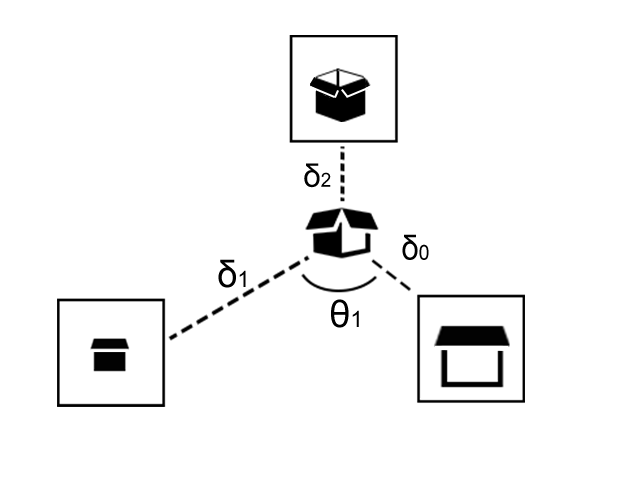
\includegraphics[width=0.4\textwidth]{object_model.png}
  \caption{Modèle polaire des objets.}
\end{figure}

Formellement, un référentiel polaire entrelace toutes ces informations
de façon à représenter la position spatiale d'où l'observation était
fait, tel comme il est représenté dans l'image *7*. Pour la
construction du modèle les conventions suivantes étaient adoptées :
\begin{itemize}
\item l'angle zéro est attribué à la première observation
\item L'origine du référentiel est la position globale de l’objet
\item Les features sont labellisées d'après le déplacement angulaire
  et la distance au centroïde de l'objet.
\end{itemize}

Une grande majorité de features visuelles sont variantes à échelle, une
fois que la résolution de l’image joue un rôle assez critique pour la
détection de features, comme les patches SIFTs. Ainsi, avoir la distance
que l’image étais prise peut être intéressant pour limiter la
classification à une échelle valable.